\documentclass[]{article}
\usepackage{graphicx}
\graphicspath{{images/}}
\usepackage[utf8]{inputenc}
\usepackage{amsmath}

% Title Page
\title{Conduction, Convection, and Radiation Analysis of an Absorber Plate for a Solar Water Heater}
\author{Caleb J. Groves}


\begin{document}
\maketitle

\begin{abstract}
\end{abstract}

\section{Introduction}

There is a strong push today to develop more environmentally-friendly ways of generating and using energy. One of the most available and interesting sources of alternative energy is solar energy. While solar energy is abundant, it tends to be of a lower grade than other forms. As such, the harvesting of this energy should be done as efficiently as possible in order to maximize the output which is needed for various applications.

This analysis compares the efficiencies of two designs for a solar water heater: one with a convection shield, and one without. The objective is to determine whether one design has a significant advantage over the other in terms of energy efficiency. The analysis is carried out using fundamental laws and principles of thermodynamics and heat transfer in order to develop a model of the solar water heater under both shielded and unshielded conditions. This model is then used to predict values for the efficiencies of the designs and give recommendations based on the results.

\section{Methods}

% General approach: identify the system, develop differential equation to model system, solve equation, solve specifically for convection and radiation terms, use given values to analyze numerically and derive results.
We define the efficiency of the solar water heater as the ratio of the rate energy is transferred to the water to the rate solar energy is incident on the absorbing surface. The general approach to analyzing the efficiencies of the two designs is as follows: the system is identified and used to develop differential equations in order to model it. This equation is then solved to obtain a the temperature profile along the absorber plate, and this temperature distribution is then used to obtain expressions for the rate energy is transferred to the water. Specific terms in these equations are solved for on a more detailed level, and then these expressions are evaluated numerically to obtain results.

\subsection{Schematic}

A general schematic for the problem is shown below in Fig. \ref{fig:base_schematic}, including values which we will assume are accurate. The solar water heater is exposed to a uniform solar flux $q''_{solar}$ at an angle $\theta$ relative to the surface normal, and quiescent air at temperature $T_{\infty}$. The bottom of the absorber plate is insulated, and the plate itself has a diffuse, spectrally selective coating with the spectral reflectivity shown in Fig. \ref{fig:base_schematic}. The water circulating through the tubes is assumed to keep the absorber plate directly above each pipe at $T_0$. We will model the surroundings as large and isothermal, also at $T_{\infty}$.

\begin{figure}[h]
	\centering
	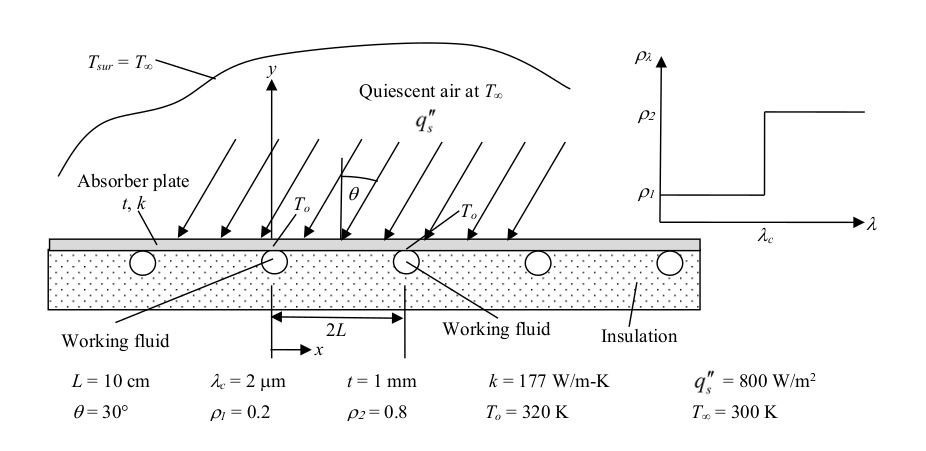
\includegraphics[width=8cm]{schematic1.png}
	\caption{Schematic of the solar water heater and its interactions with the environment.}
	\label{fig:base_schematic}
\end{figure}

\subsection{Assumptions}

Based on the information available to use from Fig. \ref{fig:base_schematic} and in order to facilitate the analysis, the following assumptions have been made:

\begin{enumerate}
	\item We will only analyze the \textit{steady-state} of the system.
	\item \label{ass:constant}The absorber plate materials can be approximated as constant - it will be shown at the end of the analysis that the temperature gradient in the is sufficiently small to justify this.
	\item There is no internal heat generation in the system - this seems reasonable, especially since no information has been given to us concerning chemical reactions or other sources of internal energy generation.
	\item Since copper is a good conductor of heat and copper water tubes are generally thin-walled, it is reasonable to neglect conduction through the tubing walls to the water.
	\item Since $t << L$, conduction in the $y$ direction can be neglected. It will later be shown in \pageref{eq:biot} further reasons as to why this assumption is reasonable.
\end{enumerate}

\subsection{Analysis}

\subsubsection{System Modeling}

Since we will need to know the temperature distribution in the absorber plate in order to determine the efficiency of the heat transfer to the water, we will choose our system to be a differential control volume in the absorber plate and model the energy interactions of this control volume with the surroundings, as shown in Fig. \ref{fig:model_schematic}.

\begin{figure}[h]
	\centering
	%\includegraphics[width=8cm]{modeling_schematic.png}
	\caption{Schematic of a differential control volume of the system of interest (the absorber plate), and the energy interactions of that system with its surroundings.}
	\label{fig:model_schematic}
\end{figure}

Identifying the interactions of this system with its surroundings shows the conduction in the $x$ direction, $q_{rad}$ out to the surroundings, $q_{solar}$ (irradiation from the sun), and $q_{conv}$. The First Law of Thermodynamics shows us:

\begin{equation} \label{eq:consv_E}
	\dot{E_{in}} - \dot{E_{out}} + \dot{E_{gen}} = \dot{E_{st}}
\end{equation}

Substituting in the pertinent interactions and assumptions into (\ref{eq:consv_E}) gives us:

\begin{equation} \label{eq:consv_2}
	(q_x + q_{solar}) - (q_{x + \Delta x} + q_{conv} + q_{rad}) = 0
\end{equation}

Let $\beta q''_{solar} A_s = q_{solar}$, where $A_s = w\Delta x$ and $\beta$ represents the fraction of $q''_{solar}$ absorbed by the system. Rearranging (\ref{eq:consv_2}) and expressing $q_{conv}$ using Newton's Law of Cooling and $q_{rad}$ using a linearized radiation coefficient gives us:

\begin{equation} \label{eq:consv_3}
	-(q_{x + \Delta x} - q_x) + \beta q''_{solar} w\Delta x - (h_{conv} + h_{rad})w\Delta x(T(\frac{x + (x + \Delta x)}{2}) - T_{\infty}) = 0
\end{equation}

Dividing (\ref{eq:consv_3}) by $\Delta x$ and taking the limit as $x$ approaches zero, we can express the first term using Fourier's Law:

\begin{equation} \label{eq:consv_4}
	\frac{d}{dx}(kA_p\frac{dT}{dx}) + \beta q''_{solar}w - (h_{conv} + h_{rad})w(T(x) - T_{\infty}) = 0
\end{equation}

where $A_p$ is the area perpendicular to the heat flux in the $x$ direction, or $wt$. Dividing (\ref{eq:consv_4}) by $w$, letting $h = h_{conv} + h_{rad}$ and using assumption (\ref{ass:constant}), we can rearrange (\ref{eq:consv_4}) as follows and obtain a differential equation modeling our system:

\begin{equation} \label{eq:model_cmplx}
	\frac{d^2 T}{dx^2} - \frac{h}{kt}T(x) = -\frac{1}{kt}(\beta q''_{solar} + hT_{\infty})
\end{equation}

Our model can be simplified by letting $m = \sqrt{\frac{h}{kt}}$ and $G = -\frac{1}{kt}(\beta q''_{solar} + hT_{\infty})$, in which case (\ref{eq:model_cmplx}) can be rearranged and written as:

\begin{equation} \label{eq:model}
	\frac{d^2 T}{dx^2} - m^2 T(x) = G
\end{equation}

Our boundary conditions are given by examining Fig. \ref{fig:base_schematic}, from which we deduce:

\begin{equation} \label{eq:boundaries}
T(0) = T_0, \quad T(2L) = T_0
\end{equation}

Thus, we gone from fundamental laws and principles describing our system in \ref{eq:consv_2} to a second-order, ordinary, linear, non-homogeneous differential equation.

\subsubsection{Model Solution}

In order to find the temperature profile $T(x)$ and solve for the heat flux to the water from the heater and subsequently the efficiencies, we will need to solve (\ref{eq:model}) subject to (\ref{eq:boundaries}). We will solve the homogeneous portion of (\ref{eq:model}) and use the method of undetermined coefficients to solve the non-homogeneous portion.

The characteristic equation of (\ref{eq:model}) is:

\begin{equation}
r^2 - m^2  = 0
\end{equation}

This corresponds to a solution of the form:

\begin{equation} \label{eq:sol_gen}
T(x) = c_1 e^{mx} + c_2 e^{-mx} + T_p(x)
\end{equation}

where $T_p(x)$ is the particular solution. If we assume $T_p(x) = A$, then we can substitute $T_p(x)$ into (\ref{eq:model}) to find that:

\begin{center}
$0 - m^2 A = G$ 
\end{center}
\begin{equation} \label{eq:A}
\begin{split}
A & = -\frac{G}{m^2} \\
& = \frac{\beta}{h}q''_{solar} + T_{\infty}
\end{split}
\end{equation}

Inserting (\ref{eq:A}) into (\ref{eq:sol_gen}), we have that the solution to (\ref{eq:model}) is:

\begin{equation} \label{eq:sol_gen1}
T(x) = c_1 e^{mx} + c_2 e^{-mx} + H
\end{equation}

where $H = \frac{\beta}{h}q''_{solar} + T_{\infty}$. The final step is to solve for $c_1$ and $c_2$. Expressing (\ref{eq:sol_gen1}) subject to (\ref{eq:boundaries}) gives us the following system of linear equations:

\begin{align*}
c_1 + c_2 & = T_0 - H \\
c_1 e^{2mL} + c_2 e^{-2mL} & = T_0 - H
\end{align*}

Solving these equations simultaneously, $c_1$ and $c_2$ are found to be

\begin{equation*}
\begin{bmatrix}
c_1\\
c_2
\end{bmatrix} = \frac{T_0 - H}{e^{-2mL} - e^{2mL}} \begin{bmatrix}
e^{-2mL}-1 \\
1-e^{2mL}
\end{bmatrix}
\end{equation*}

Using these results, (\ref{eq:sol_gen1}) can now be expressed as

\begin{equation} \label{eq:long_T}
T(x) = \frac{T_0 - H}{e^{-2mL} - e^{2mL}}[(e^{-2mL}-1)e^{mx} - (e^{2mL}-1)e^{-mx}] + H
\end{equation}

It can be shown that equation~(\ref{eq:long_T}) can be simplified using the hyperbolic function definitions, until we arrive at the following equation for the temperature distribution:

\begin{equation} \label{eq:T}
\boldsymbol{T(x) = \frac{T_0 - H}{\cosh(mL)}\cosh(m(x-L)) + H}
\end{equation}

Equation~(\ref{eq:T}) is therefore the mathematical solution for the temperature distribution of the absorber plate, from one copper tube to the next. It is dependent, of course, on the quantities $m$ and $H$, which, as a reminder, are given by (\ref{eq:m}) and (\ref{eq:H}) below:

\begin{equation} \label{eq:m}
m \equiv \sqrt{\frac{h}{kt}}
\end{equation}

\begin{equation} \label{eq:H}
H \equiv \frac{\beta}{h}q''_{solar} + T_{\infty} \\
h \equiv h_{conv} + h_{rad}
\end{equation}

\section{Results}

\section{Discussion}

\end{document}          
